\documentclass[11pt,reqno]{article}
\newcommand{\vet}[1]{{\ensuremath{\mbox{\boldmath $#1$}}}}
\renewcommand{\baselinestretch}{1.5}
\setlength{\oddsidemargin}{0in} \setlength{\textwidth}{6in}
\setlength{\topmargin}{-0.2in} \setlength{\textheight}{8.8in}
\def\labelitemi{--}
\usepackage{graphicx}
\usepackage{amsmath}
\usepackage[T1]{fontenc}
\usepackage{lmodern}
\usepackage{amssymb,amsmath}
\usepackage[style=apa]{biblatex}
\usepackage[linkcolor=blue]{hyperref}
\usepackage[title]{appendix}
\usepackage{xurl}
\usepackage{booktabs}
\addbibresource{bes.bib}



\begin{document}

\titlepage
\title{\textbf{Bayesian Evidence Synthesis for Informative Hypotheses: An introduction}}
\author{\textbf{Irene Klugkist, Thom Benjamin Volker} \\
Methodology and Statistics, Social and Behavioral Sciences, Utrecht University} \maketitle



\noindent \textbf{Abstract}

\noindent To establish a theory one needs cleverly designed and well executed studies with appropriate and correctly interpreted statistical analyses. Equally important, one also needs replications of such studies and a way to combine the results of several replications into an accumulated state of knowledge. An approach that provides an appropriate and powerful analysis for studies targeting pre-specified theories is the use of Bayesian model selection for informative hypotheses. Furthermore, it is claimed that an additional advantage of the use of this Bayesian approach is that combining the results from multiple studies is straightforward. In this paper we discuss the behavior of Bayes factors in the context of evaluating informative hypotheses with multiple studies. By using simple models and (partly) analytical solutions we compare two approaches to combine evidence of multiple studies: Bayesian Evidence Synthesis with Bayesian Sequential Updating. By doing so we clarify how different replication or updating questions can be evaluated. In addition, we illustrate Bayesian Evidence Synthesis with two simulations, in which multiple studies are generated to resemble conceptual replications. In this situation, the studies are too heterogeneous to be aggregated with conventional research synthesis methods, such as Bayesian Sequential Updating.


\bigskip

\noindent Keywords and phrases: Bayesian evidence synthesis, Bayes factors, Bayesian updating, Informative hypotheses, Replication


\newpage

\section{Introduction}
\label{intro}


For any empirical science, replicability is an essential topic. There are several papers on the need for replication, including explanations on reasons for lack of replication studies and recommendations on how to increase replicability \autocite{asendorpf_replication_2013, simonsohn_telescopes_2015, verhagen_bayesian_2014, nosek_replicability_review_2021}.
Especially, the replication crisis in psychology (and other fields) initiated several initiatives in this area, for instance, the Reproducibility Project \autocite{open_science_collab_2015, open_science_collab_2012} and the Registered Replication Reports initiative \autocite{simons_registered_2014}. Also, several journals are devoted to, or reserve specific sections of their journal for reports of replication studies (e.g., Royal Society Open Science, Journal of Personality and Social Psychology, Archives of Scientific Psychology, Journal of Experimental Psychology: General).

It is important to distinguish between different types of replication studies, based on how similar the studies are in their design. \textit{Direct}, \textit{close} or \textit{exact replications} aim for as much similarity with the original study as possible, such that the only difference is that in the replication study new data has been collected \autocite{simons_direct_2014, brandt_et_al_replication_2014}. Aggregation of results from exact replications is relatively straightforward. If a study is a strictly exact replication of the initial study and the raw data from both studies are available, then the data can be combined and analyzed as if it was one large study. In practice, usually other approaches are used, for instance, within the Bayesian framework, one could apply Bayesian sequential updating \autocite{schonbrodt_sequential_2017}. This provides a summary of results after the initial study, an updated summary after adding one replication, a further updated summary after adding another replication, and so forth. The final result of Bayesian updating of data from multiple studies is exactly the same as the result of one Bayesian analysis of all data combined, as long as the same initial prior is used.

Another common approach to aggregation of multiple studies is (Bayesian) meta-analysis \autocite[see][]{lipsey_wilson_2001, sutton_bayesian_meta2001}. One advantage of the meta-analysis approach is that one does not need the raw data of the studies. The aggregation is at the level of summary statistics (e.g., effect sizes and standard errors) which are often available in the publications of the separate studies. Another difference making meta-analysis more flexible is that studies do not have to be strictly exact replications. With random effects meta-analysis and the option of adding moderators to explain differences between studies, the model accounts for and potentially helps understanding heterogeneity in the results. Still, aggregating results using meta-analysis requires a relatively high level of similarity between studies. Since the aggregation is at the level of effect sizes, comparable effect sizes must be available for all studies to be synthesized. For studies that are theoretically related but methodologically highly diverse meta-analyzing the results may not be feasible.

In the context of \textit{indirect} or \textit{conceptual replications} the studies may indeed be highly diverse. One common theory may be investigated in different contexts, with different study designs, using different instruments, variables, and statistical analyses. An advantage of performing conceptual replications is that results that agree across different methodologies and contexts jointly provide stronger support for the underlying central theory \autocite{crandall_conceptual_2016, lawlor_triangulation_2017, nosek_scientific_2012}. A disadvantage is that the aggregation of results of conceptual replications is not straightforward.

\textcite{kuiper_combining_2013} proposed a method based on combining evidence for informative hypotheses on the level of Bayes factors. The underlying idea is that the central theory of interest is allowed to be operationalized differently in each study. The study specific informative hypothesis, that represents the central theory, is evaluated using the Bayes factor, which measures the support in the data for the hypothesis of interest against some alternative. Stated differently, the Bayes factor quantifies, based on the observed data, the change from the prior odds of two competing hypotheses to the posterior odds of those hypotheses. Aggregation of evidence from multiple studies is done by using the posterior odds after the first data set as the prior odds for the next (i.e., a replication study). This provides updated (with each new replication) relative support measures for the two hypotheses that are compared.

Using this approach, each study provides a level of evidence for the central theory despite the diversity in study design. Although it has been applied successfully \autocite{zondervan_parental_2019, zondervan_robust_2020, kevenaar_bes_2021, volker_cooperation_2022}, a paper describing the correct interpretation of the combined evidence and the advantages and limitations of this approach is currently lacking. The main goal of this article is therefore to provide a clear and correct understanding of this Bayesian Evidence Synthesis (BES) approach, that is based on combining Bayes factors that result from evaluating informative hypotheses.

In the next section, we demonstrate the behavior of Bayes factors for an inequality constrained hypothesis in one study. The use of Bayesian model selection for informative hypotheses is shortly outlined and the Bayes factor is introduced using a simple binomial example. Subsequently, we consider the synthesis of results from multiple studies. The starting point is an example where a set of exact replications is available, again using the binomial model as illustration. This is followed by an example in the context of conceptual replications, where BES is applied to a set of highly diverse studies in simulations. The paper ends with a discussion of results and recommendations for potential users of BES, as well as for future methodological research. All materials to reproduce these examples can be found on GitHub \autocite{Klugkist & Volker, 2022a}.




\section{Bayes factors for informative hypotheses in one study}
\label{theory}

Informative hypotheses are hypotheses that impose inequality and equality constraints on model parameters to reflect specific expectations that researchers may have when designing their study. Some background on the motivation to use informative hypotheses is provided in the first subsection. A summary of the approach for the evaluation of informative hypotheses using Bayes factors is provided next. This approach has been proven useful and intuitive, and has been described, investigated and applied for the analysis of single studies extensively in the past two decades \autocite{beland2012informative, hoijtink_tutorial_2019, mulder_prior_2014, flore_influence_2018, gu_inequality_2014}. In the final subsection, a binomial example illustrates the approach. With this simple model, analytical solutions are available for the Bayes factors of interest. The conclusions from the binomial example, however, also extend to other examples and statistical models.


\subsection{Informative hypotheses}\label{inf_hyp}

Researchers often initiate their study with specific expectations or theories about the outcomes in mind. For instance, in an experimental design, specific conditions are included because it is \emph{a priori} expected that in certain conditions participants will score higher or lower than in other conditions. Such expectations are naturally represented by order constraints on the model parameters. As an example, consider a study that compares the effectiveness of two treatments and one control condition. The expectation of the researcher is that treatment $A$ will lead to, on average, higher outcome scores than treatment $B$, but both treatments are expected to be more effective, and thus score higher, on average, than the control group $C$. With $\mu_j$ denoting the group mean of group $j$ ($j = A, B, C$), this can be expressed as the informative hypothesis:
\[H_i: \mu_A > \mu_B > \mu_C.\]
Informative hypotheses can also include equality constraints. A researcher could, for instance, state the expectation that treatment A and B are equally successful and that both are better than control condition C, that is: $(\mu_A = \mu_B) > \mu_C$. In addition, specific interaction patterns can also be expressed using inequality and equality constraints. For instance, in a $2\times2$ design investigating a treatment (T) versus control (C) effect for both males (M) and females (F), the expectation that the treatment is effective for all, but more effective for males, could be expressed as:
\[H_i: \mu_{TM} > \mu_{CM} \mbox{ and } \mu_{TF} > \mu_{CF} \mbox{ and } (\mu_{TM}-\mu_{CM}) > (\mu_{TF}-\mu_{CF}).\]
For examples of applications of informative hypothesis evaluation in psychology, for instance, see: \textcite{cooper_relationship_2014, bullens_role_2011, vanuijlen_approach_behavior_2017, matthijssen_effects_2019}.


There are several reasons why a traditional null hypothesis test based on $p$-values is not the optimal choice for the evaluation of informative hypotheses. First of all, the hypotheses included in the NHT approach are often not the research hypothesis of interest. Several authors claimed that the null hypothesis can never be (exactly) true \autocite[e.g.,][]{cohen_earth_1994, krueger_null_2001, lykken_wrong_1991} and therefore rejecting it does not tell us anything. In addition, the alternative hypothesis in NHT is not specific or informative (usually just stating 'not $H_0$'). \textcite{royall1997statistical} argues that the focus of a statistical analysis should not be on the question whether there is evidence against the null hypothesis but, instead, one should ask whether there are scientifically meaningful alternative hypotheses that are better supported \autocite[][p. 81]{royall1997statistical}.

An informative hypothesis is an example of a scientifically meaningful hypothesis. If one would evaluate it using the NHT approach follow-up tests like pairwise comparisons are required. How to control type 1 and 2 errors in the resulting multiple testing situation is not at all straightforward \autocite[e.g.,][]{maxwell_persistence_2004}. There is a risk of over-interpreting patterns in the observed data that are not necessarily indicative for patterns in the population, but resemble noise that is unique to the data at hand. Some researcher may even be tempted to HARKing \autocite[Hypothesizing After Results are Known;][]{kerr_harking_1998}, as if the observed patterns were the anticipated results patterns a priori. Finally, the power to find support for an informative hypothesis using NHT with follow-up testing is extremely low \autocite{klugkist_confirmatory_2014}.
A final argument against NHT is that researchers want to know how much support the data provide for their hypothesis. However, the $p$-value resulting from NHT is not the probability that any hypothesis is true or false and therefore does not provide such information \autocite[e.g.,][]{cohen_earth_1994}. A better alternative for testing informative hypotheses has been found within the Bayesian framework and is presented in the next section.




\subsection{Bayesian model selection}
\label{BMS}

Bayesian model selection can be used for the evaluation of informative hypotheses and is based on the Bayes factor. There are many references that explain the Bayes factor in general \autocite{kass_raftery_bayes_factors_1995, hoijtink_tutorial_2019, heck_review_2022} as well as in the specific context of testing informative hypotheses \autocite[e.g.,][]{beland2012informative, klugkist_inequality_2005, gu_inequality_2014, hoijtink_informative_2012}. Shortly summarized, the Bayes factor compares two models or hypotheses $H_1$ and $H_2$, by:
\begin{equation*}
  BF_{1,2} = \frac{P(D|H_1)}{P(D|H_2)},
\end{equation*}

\noindent where $P(D|H_1)$ and $P(D|H_2)$ denote the probability that the data was generated under $H_1$ versus the probability that the data was generated under $H_2$. So, when the resulting value is larger than one, there is more support for $H_1$, whereas $BF_{1,2}<1$ implies more support for $H_2$.

To evaluate an informative hypothesis with a Bayes factor it is required to formulate at least one alternative hypothesis. In the context of informative hypotheses we investigate three natural choices: the unconstrained alternative, the complement of the informative hypothesis, and the null hypothesis. In the following subsections, each of the options and some of their strengths and limitations are discussed.



\subsubsection{Testing against the unconstrained model}
From here, let the interest be to evaluate if and to what extent the data support the expectation $H_i: \mu_A > \mu_B > \mu_C$.
Testing against the unconstrained alternative $H_u: \mu_A, \mu_B, \mu_C$ is proposed by \textcite{klugkist_inequality_2005}, but see also \textcite{hoijtink_informative_2012} and \textcite{hoijtink_klugkist_boelen_2008}. It represents how the Bayes factor computation for informative hypotheses is implemented in what is called the encompassing prior approach. Each informative hypothesis can be seen as the unconstrained hypothesis plus a set of constraints. The encompassing prior approach uses this property by deriving an expression for the Bayes factor, $BF_{i,u}$, that requires only evaluation of the unconstrained model and determining the part of it that is in agreement with the constraints. Such evaluation of the posterior distribution of the parameters provides a measure of relative fit for the constrained versus the unconstrained model (denoted $f_i$). A similar evaluation of the prior distribution is required to determine the relative size, or complexity, of the constrained model (denoted $c_i$). The latter shows that a Bayes factor incorporates an automatic correction for model size to prevent from overfitting. Evaluation of prior and posterior distributions can sometimes be done analytically \autocite[e.g.,][]{mulder_gu_bayesian_2021}. If this is not possible, evaluation is possible through  Markov chain Monte Carlo (MCMC) sampling \autocite{gilks_markov_1995}. The resulting estimate of the Bayes factor is:

\begin{equation}\label{BFfc}
  BF_{i,u} = \frac{f_i}{c_i}.
\end{equation}

Evaluating hypotheses that include equality constraints using the encompassing prior approach requires some additional steps \autocite[see][]{klugkist_inequality_2005, vanwesel_choosing_2011, mulder_equality_2010} and will not be further discussed at this point. Finally, note that researchers may have multiple, competing informative hypotheses, say $H_{1}$ and $H_{2}$. The Bayes factor that mutually compares two informative hypotheses, that is, $BF_{1,2}$, is then easily computed by applying (\ref{BFfc}) twice providing $BF_{1,u}$ and $BF_{2,u}$ and the notion that:

\begin{equation*}
  \frac{BF_{1,u}}{BF_{2,u}} = \frac{P(D|H_{1}) / P(D|H_u)}{P(D|H_{2}) / P(D|H_u)} = \frac{P(D|H_{1})}{P(D|H_{2})} = BF_{1,2}.
\end{equation*}


\subsubsection{Testing against the complementary model}
Testing against the complement of a constrained hypothesis is described by \textcite{hoijtink_informative_2012}, but see also \textcite{vandeun_testing_2009} and \textcite{vanrossum_hypothesis_2013}. It provides the most powerful test when the interest lies in \emph{one} informative hypothesis, because the two hypotheses describe mutually exclusive situations. For $H_i: \mu_A > \mu_B > \mu_C$, the complement $H_c$ is the collection of all orderings of means that is not $H_i$.
A potential disadvantage is that it is not straightforward to define the complement of a hypothesis including equality constraints. Pragmatically, \textcite{gu_approximated_2018} propose that the unconstrained model ($H_u$) serves as the complement for any hypothesis that includes at least one equality constraint. In this paper, we limit the examples and simulations to an informative hypothesis that imposes inequality constraints on parameters, in which case the complement is clearly defined as 'any ordering other than the one specified in $H_i$'.

The computation of the Bayes factor comparing an order constrained hypothesis $H_i$ with its complement $H_c$ follows easily from (\ref{BFfc}) and the notion that the fit of the complement $f_c$ equals $1-f_i$ and the complexity of the complement $c_c$ equals $1-c_i$. This provides:
\begin{equation}\label{BFic}
  BF_{i,c} = \frac{BF_{i,u}}{BF_{c,u}} = \frac{f_i / c_i}{(1-f_i)/(1-c_i)}.
\end{equation}


\subsubsection{Testing against the null model}
The third option is testing the informative hypothesis against the null hypothesis $H_0: \mu_A = \mu_B = \mu_C$. Since the null hypothesis is considered unrealistic ('the exact null is never true') and usually does not represent a theoretical expectation of the researcher, it could be argued that it is not a good competitor for the informative hypothesis. However, often researchers prefer to include and evaluate the option that all sample effects are likely to be chance results and therefore want to compare the theoretical expectation with the model stating that there are no effects at all.
The Bayes factor of $H_0$ against the unconstrained model ($BF_{0,u}$) can also be estimated with (\ref{BFfc}), but an adjustment is necessary to estimate the fit $f_0$ and complexity $c_0$ for the null hypothesis. Technical details and a thorough investigation of the performance of the proposed estimator can be found in, for instance, \textcite{mulder_equality_2010}. Another approach for the estimation of $BF_{0,u}$ is the Savage-Dicky density ratio method as explained by \textcite{wagenmakers_bayesian_2010}. This approach computes the ratio of the posterior density and the prior density at the hypothesized value of the parameter(s) and is applied in the binomial example in this paper.

From the estimated $BF_{0,u}$ one can easily derive the Bayes factor of interest that compares $H_i$ with $H_0$ using:
\begin{equation*}
  BF_{i,0}=\frac{BF_{i,u}}{BF_{0,u}}.
\end{equation*}
Note that when evaluating the null hypothesis, or any informative hypothesis that includes one or more equality constraints, the results can be highly sensitive to the choice of the (encompassing) prior.
Recently, \textcite{hoijtink_prior_2021} provided a comprehensive overview of ways to deal with such prior sensitivity. 
Yet, the focus of this paper is not on the effect of the prior on the resulting Bayes factor, but on the behavior of Bayes factors in replication. In the analyses of this paper we state which prior we used but we do not investigate the sensitivity of results to that choice.


\subsubsection{Posterior model probabilities}

So far, we provided equations for the computation of Bayes factors. Results can, however, also be expressed in terms of posterior model probabilities. The ratio of two posterior model probabilities (i.e., posterior odds) is computed by taking the product of the ratio of the prior model probabilities (i.e., prior odds) and the Bayes factor. We usually assume both hypotheses equally likely before observing any data, that is, the prior odds equal one. In that case, the posterior model probabilities reflect the same information as the Bayes factor but are re-scaled to a score between zero and one, where a larger score means more support for the hypothesis. To give just one example, $BF_{1,2}=3$ expresses that the support in the data for $H_1$ is 3 times higher than the support for $H_2$. With equal prior model probabilities for $H_1$ and $H_2$, this leads to posterior model probabilities of 0.75 for $H_1$ and 0.25 for $H_2$.



\subsection{Bayes factors for a Binomial example}\label{Singlestudy}


A simple example of an inequality constrained hypothesis is testing a success probability $\theta$ based on the number of successes $x$ in a sample of $n$ trials assuming $x \sim Bin(n, \theta)$, that is, a binomial distribution:
\begin{equation}\label{binlik}
  f(\theta|n, x) = \binom{n}{x}\theta^x(1-\theta)^{n-x}.
\end{equation}

\noindent It is convenient to use the conjugate beta prior:

\begin{equation}\label{betaprior}
  p(\theta|\alpha, \beta) = \frac{1}{B(\alpha, \beta)} \theta^{\alpha-1}(1-\theta)^{\beta-1},
\end{equation}
where $B(\alpha, \beta)$ denotes the beta function.
We use (\ref{betaprior}) with $\alpha=\beta=1$ as the prior distribution for a success probability $\theta$ without any constraints imposed, that is,  $H_u: \theta$. This is equal to the uniform distribution on the interval [0,1], i.e. $p(\theta) = 1$. With this choice one states that, a priori, each value for $\theta$ between zero and one is considered equally likely.

The unconstrained posterior distribution using the binomial likelihood and the $Beta(\alpha,\beta)$ prior is $Beta(\alpha+x, \beta+n-x)$. For the $Beta(1,1)$ prior this reduces to the $Beta(x+1, n-x+1)$ posterior distribution. It is easy to see that this distribution equals the likelihood in (\ref{binlik}), that is, the constant prior does not add any information about $\theta$, and therefore the posterior is determined by the data only.

\begin{figure}[ht]
 \centerline{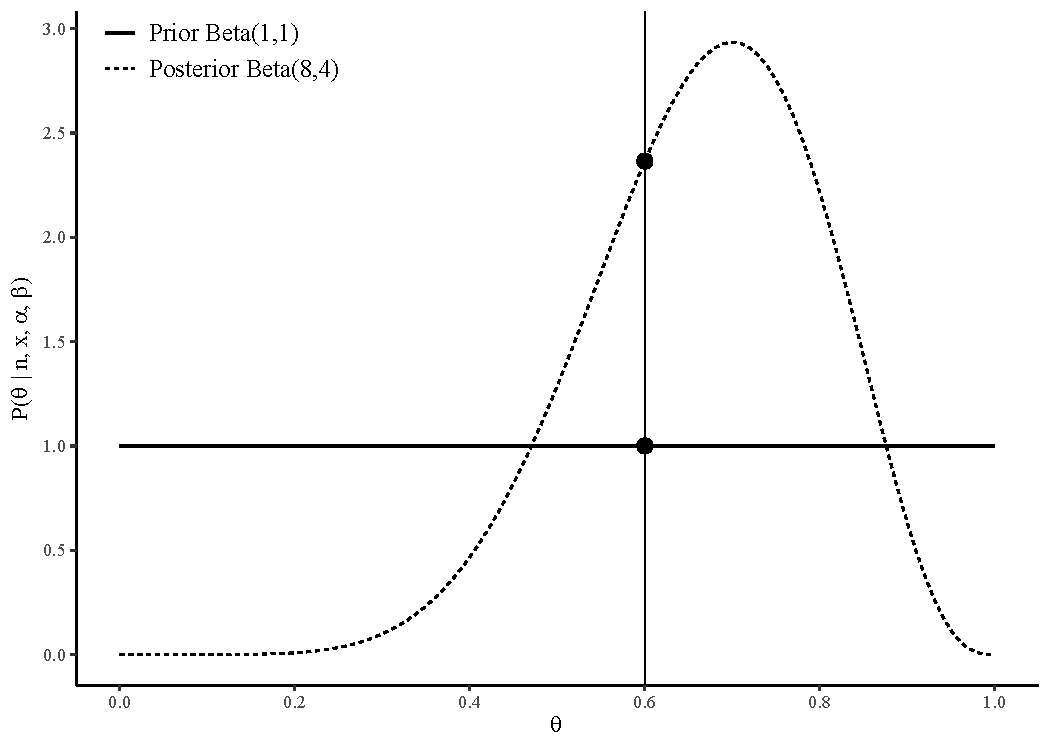
\includegraphics[width=12cm]{r-files-bes-klugkist-volker-2022/Figures/betaplot}}
 \caption{Prior $Beta(1,1)$ and the Posterior $Beta(8,4)$ after observing 7 successes in a sample of size 10.}
 \label{betaplot}
\end{figure}

To illustrate inequality constrained testing, we consider the hypothesis stating that the success probability is larger than 0.6.
This hypothesis is evaluated against the unconstrained, the complement, and the null hypothesis. In this relatively simple model, the Bayes factors can be computed analytically instead of through MCMC sampling from the prior and posterior distributions. Using Figure \ref{betaplot}, the calculation of each Bayes factor is explained. The plot shows the prior distribution, $Beta(1,1)$, as well as a posterior assuming that we observed a sample of size $n=10$ with number of successes $x=7$, providing $Beta(8,4)$.

\begin{table}[!h]
\caption{Posterior fit $f_j$ (for $H_i$ and $H_c$) or density at $\theta=0.6$ (for $H_0$), prior fit $c_j$ (for $H_i$ and $H_c$) or density at $\theta=0.6$ (for $H_0$) and Bayes factor for each hypothesis against $H_u$ (based on $Beta(1,1)$ prior for $\theta$ and $x=7$ successes in $n=10$ observations)}
\label{calcBF}
  \centering
     \begin{tabular}{lrrr}\hline
$H_j$                 & posterior   & prior  & $BF_{j,u}$   \\ \hline
$H_u: \theta$        & 1     & 1     & 1       \\
$H_i: \theta>0.6$    & .704  & .400  & 1.76    \\
$H_c: \theta<0.6$    & .296  & .600  & 0.49    \\
$H_0: \theta=0.6$    & 2.365 & 1.00  & 2.36    \\ \hline
\end{tabular}
\end{table}


For $BF_{i,u}$ and $BF_{c,u}$ we need to evaluate the parts of both the prior and the posterior distributions in agreement with the constraints of $H_i$ and $H_c$, respectively. The volume of the Beta distribution that is in line with the constraints can, for instance, be calculated using the \verb"pbeta" function in \verb"R".
For $BF_{0,u}$ we use the Savage-Dickey density ratio method. In Figure \ref{betaplot}, the two large dots show the two densities that are required for this ratio: the prior and posterior density at $\theta=0.6$. These densities can, for instance, be obtained by the \verb"R" function \verb"dbeta". The resulting values for fit, complexity and the Bayes factor against the unconstrained model are provided in Table \ref{calcBF}.

From these results, the Bayes factors of interest (for $H_i$ against each of the alternatives) can easily be computed, as was explained before.
In Table \ref{Neffect}, the first column provides the results for the current scenario ($n=10$, $x=7$). The other columns, demonstrate the behaviour of the different Bayes factors for increasing sample size (with the success rate fixed at 0.7 and thus in agreement with the hypothesis of interest $H_i$).


\begin{table}[!h]
\caption{Testing $H_i: \theta>0.6$ against $H_u$, $H_c$, and $H_0$ for increasing sample sizes $n$ and fixed observed success probability ($x/n=0.7$); all with prior $p(\theta)\sim Beta(1,1)$}
\label{Neffect}
  \centering
     \begin{tabular}{crrrrrrr}\hline
             & 10    & 20    & 40   & 80   & 100  & 500  & 1000  \\ \hline
 $BF_{i,u}$  & 1.76  & 2.00  & 2.24 & 2.41 & 2.45 & 2.50 & 2.50  \\
 $BF_{i,c}$  & 3.56  & 5.99  & 12.72& 41.53& 70.69& 8.2E5  & 5.6E10   \\
 $BF_{i,0}$  & 0.74  & 0.77  & 0.95 & 1.73 & 2.42 & 6.3E3  & 2.2E8   \\ \hline
\end{tabular}
\end{table}

The results show that all three Bayes factors generally behave well with increasing support for $H_i$ when the sample size increases. However, we also see that $BF_{i,u}$ is bounded at a maximum of 2.50. The explanation is straightforward when considering the formula $BF_{i,u}=f_i/c_i$. With a result in agreement with $H_i$ and increasing sample size, at some point the entire posterior is in agreement with $H_i$, providing $f_i=1$, i.e., the maximum value for perfect fit. The Bayes factor is then determined by the complexity measure $c_i$ that does not depend on sample size and is equal to 0.4 in our example. The maximum $BF_{i,u}$ value is then 1/0.4 = 2.50.

Another observation is that testing against the null hypothesis suffers from `power' problems when samples are small. In this example, for samples of 10, 20, or 40 observations, $BF_{i,0} < 1$, showing more support for $H_0$ than for $H_i$. The explanation is simple and very similar to what happens with NHT in the frequentist framework: the parsimoniousness of the null hypothesis (it has less parameters than any of the other models) benefits this model when deviations from the null are small compared to the amount of evidence (i.e., the sample size of the study).

These observations lead us to two general recommendations for two different situations. First, if the main goal is to evaluate one informative hypothesis and to what extent it is supported by the data, then it is recommended to use $BF_{i,c}$. It is the most powerful test and it does not have a maximum value, so, the more data in agreement with the hypothesis are observed, the more support the Bayes factor will show. Second, if multiple informative hypotheses are of interest, and specifically their mutual comparison, it is recommended to evaluate them against one another. One of these informative hypotheses could also be the null hypothesis but, when including the null, one needs to take into account that a sufficient sample size is required to have reasonable power to detect the true hypothesis if this is not the null. Whether a sample is sufficiently large depends on the number of parameters and the number and type of constraints and is, to the best of our knowledge, hardly studied \autocite[for an exception in the context of comparing 2 means, see][]{fu_sample_2021}.



\section{Aggregating evidence from multiple studies}\label{Multiple}

Replication is important and increasingly performed but it raises the question of how to aggregate results from multiple studies. We discuss and compare two Bayesian options: Bayesian sequential updating (BSU) and updating at the level of Bayes factors (BES). In the context of exact replications, i.e., for data sets that have the same format, both can be applied but will give different results. In the first subsection this is discussed conceptually and in the next subsection the differences are illustrated using the binomial example again. The final subsection provides an illustration of the synthesis of evidence from a set of \textit{conceptual} replications. The studies to be synthesized come from the same underlying population (with known effect size) but consist of different data formats, that are therefore analyzed by different statistical models. Aggregation of these studies is not feasible with BSU. Using an example with different types of regression models as the statistical analysis tools, we demonstrate that the BES approach does provide a measure for the combined amount of evidence. A few simulation studies are presented to get a first impression of what BES entails, how it works, and what potential limitations are.


\subsection{Two updating schemes for exact replications}\label{Twomethods}

\subsubsection{Bayesian sequential updating (BSU)}
BSU has been well described in the literature \autocite[e.g.,][]{schonbrodt_sequential_2017, verhagen_bayesian_2014} and is a procedure that pools data either case by case or study by study. The key idea is that the current state of knowledge about a parameter or hypothesis can be computed at any moment in the data collection period. In the context of replication, data from a first study provides (after specifying an initial prior) the posterior distribution, which is subsequently used as the prior distribution for a second study. After each study, the posterior reflects the current state of knowledge about the model parameters. Also, after each study, Bayes factors can be computed and reflect the current level of relative evidence for the hypotheses of interest.

It is important to note that, with the same initial prior distribution, the posterior after adding one set of 100 observations is exactly the same as the posterior after sequential updating, for instance, after every tenth observation. Also the order in which (subsets) of data come in does not affect the final result. Finally, in contrast with the NHT approach, no penalty for multiple testing is required when computing the Bayes factor after each updating step \autocite{schonbrodt_sequential_2017}.

Sequential updating has some strengths and limitations. A first strength (compared to the NHT approach) is that a priori power analyses are not needed. Instead, one can specify a stopping rule, e.g., \textit{the resulting Bayes factor should be larger than 10 for one of the two compared hypotheses}. Data collection and evaluation of the hypotheses then continues until this threshold is reached (or resources are exhausted). A second strength is that by pooling the data from multiple studies the overall power to detect true effects increases. Especially when the null hypothesis is included as a hypothesis of interest, with small samples there may be limited power to detect relatively small effects. Data pooling increases the overall power to detect non-null effects.
The limitation of sequential updating is the high level of similarity that the studies to be aggregated must have. To use data pooling techniques (sequential updating is one example, meta-analysis another), the data must have a similar format, because the synthesis takes place at the level of the model parameters or functions of parameters, like effect sizes. For highly diverse studies like those that could result from conceptual replications, we need a more flexible approach.


\subsubsection{Bayesian evidence synthesis (BES)}

BES aggregates evidence from multiple studies at the level of Bayes factors instead of on the level of (functions of) parameters. The synthesis of evidence is based on updating model probabilities using:
\begin{equation}\label{odds}
  \frac{P(H_1|D)}{P(H_2|D)}=\frac{P(H_1)}{P(H_2)}BF_{1,2}.
\end{equation}
This equation states that the posterior odds of two hypotheses is obtained by updating the prior odds of these hypotheses with the Bayes factor, reflecting the information in the data. 
Subsequently, the posterior odds after observing a first data set can be used as the prior odds for new data. The Bayes factor measuring the evidence for the hypotheses of interest in the second data set then again updates these prior odds to posterior odds. This process can be repeated for each new data set, or each additional replication study.

In conceptual replications, a common theory of interest is investigated with studies that have substantial differences. As stated before, this diversity between studies makes data pooling complex or even impossible, because the studies provide data sets of different formats and apply models with different parameters. This diversity will also lead to different, study-specific informative hypotheses. However, given that for each study the informative hypothesis does reflect the common theory of interest, Bayes factors can be computed for each study and meaningfully aggregated.

It is important to note that the described BES approach is \emph{not} a data pooling approach. It is a flexible tool for evidence synthesis but it measures combined evidence in a different way, compared to data pooling methods like BSU or meta-analysis. 
Whereas the latter investigates to what extent all data together (`pooled') provide evidence, BES investigates to what extent the hypothesis of interest is supported over \emph{all studies}. 
That is, BES quantifies the evidence for or against the hypothesis of interest in each individual study and then pools the evidence over studies, providing a joint level of support for the general theory. The different methods for aggregating evidence from multiple studies lead to different results when applied to the same data. This is illustrated in the next subsection.


The fact that BES is not a data-pooling method can be seen as a limitation of the approach, because one of the goals of aggregating over multiple studies may be to increase the power to find support for a hypothesized effect, especially when the individual studies are relatively small. BES does not solve power problems because it does not measure support in pooled data. However, in the context of conceptual replications the BES approach fits very well and provides answers to a useful question, that is, what is the overall, combined level of support for a hypothesis when investigated with studies that are related but not similar.
If the hypothesized effect finds support in each of these studies, then it can be concluded that the results are robust with respect to (perhaps arbitrary) study design choices. So, BES provides a flexible tool that can synthesize evidence from studies that may be highly diverse and it answers a research question that is relevant for conceptual replications and enables robust scientific conclusions.



\subsection{Aggregation in the binomial example}\label{Binmultiple}

For the binomial example, and under the assumption that we have exact replications, we compare results from aggregation using BSU and BES. We evaluate the informative hypothesis $H_i: \theta>0.6$ by aggregating evidence from 1 to 5 studies, where each study has a sample size of 20 and an observed success probability of 0.7. As in the previous example, we use a $Beta(1,1)$ prior distribution. In Figure \ref{Aggregated}, the evaluation of $H_i$ against one of three alternative hypotheses is presented: the unconstrained model $H_u: \theta$ (left panel), the complementary model $H_c: \theta<0.6$ (centre panel), and the null model $H_0: \theta=0.6$ (right panel). Results are presented as posterior model probabilities (PMP) for $H_i$ after each additional study, using equal initial prior model probabilities.


\begin{figure}[ht]
   \centerline{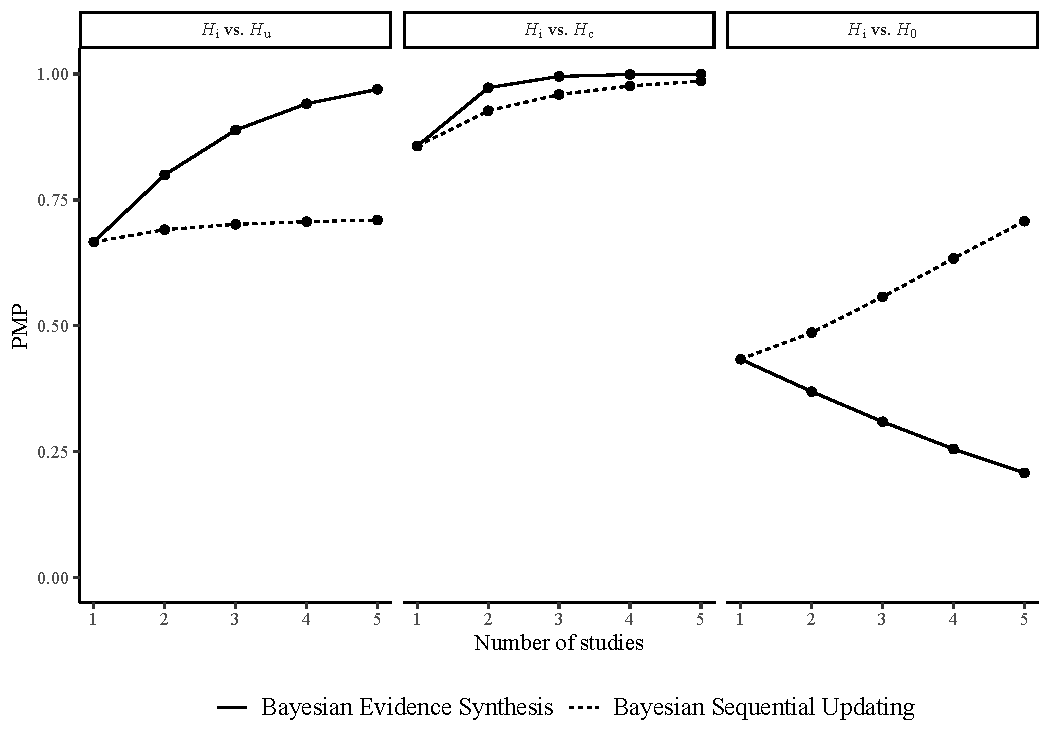
\includegraphics[width=14cm]{r-files-bes-klugkist-volker-2022/Figures/bes_bsu_7_pmp}}
 \caption{PMPs for BES (solid lines) and BSU (dashed lines) after combining 1-5 studies of $n=20$ and $x/n=0.7$ per study. All PMPs are the result of evaluating $H_i: \theta>0.6$ against one of the alternatives. Left panel: $H_u: \theta$. Centre panel: $H_c: \theta<0.6$. Right panel: $H_0: \theta=0.6$.}
 \label{Aggregated}
\end{figure}


It is clear that the two approaches provide different results. When testing against the unconstrained model, BSU `suffers' from the fact that the BF has a maximum. When there is enough evidence to reach a fit-value of one, the BF per study can not further increase than 1/complexity; in our example 1/0.4=2.5 (PMP=0.71), which explains the almost horizontal dashed line in the first panel (on the left). Instead, BES aggregates the amount of support for $H_i$ versus the alternatives in each study. Since every single study shows a preference for $H_i$ compared to $H_u$ ($BF_{i,u}=2$), the synthesized evidence for $H_i$ over multiple studies increases with each additional study, as can be seen by the steadily increasing solid line in this plot. In the second plot (centre), both synthesis methods show an increase in the aggregated PMP with an increasing number of studies that support $H_i$. Again the differences in results between the approaches are caused by the fact that a different synthesis question is answered. This becomes even clearer in the right-hand panel, where $H_i$ is evaluated against $H_0$, while each individual study does not have enough power to show preference for $H_i$ over the more parsimonious model $H_0$. In this scenario, BSU shows an increasing amount of evidence for $H_i$ when adding additional studies. The data pooling approach achieves that at some point there is enough power to find more support for the informative hypothesis than for the null hypothesis. This is not the case for BES, because the question answered by BES is about the support for $H_i$ in each individual study. Because each individual study prefers the simpler $H_0$, the aggregated evidence for $H_0$ becomes stronger with each additional study. This explains the decreasing solid line for the declining support for $H_i$.

To get further insight in the behaviour of aggregated evidence using BSU and BES, similar plots are constructed for data with different success probabilities. We start with a sample success rate of 0.8, i.e., again supporting the informative hypothesis of interest, but with more power due to a larger effect. Then we investigate results when the sample supports the null hypothesis, that is, a success rate of 0.6, and finally when the complement is supported with a success rate of 0.4. The same prior specifications are used, each study still has a sample size of n=20, and 5 identical studies are aggregated.


\begin{figure}[!ht]
   \centerline{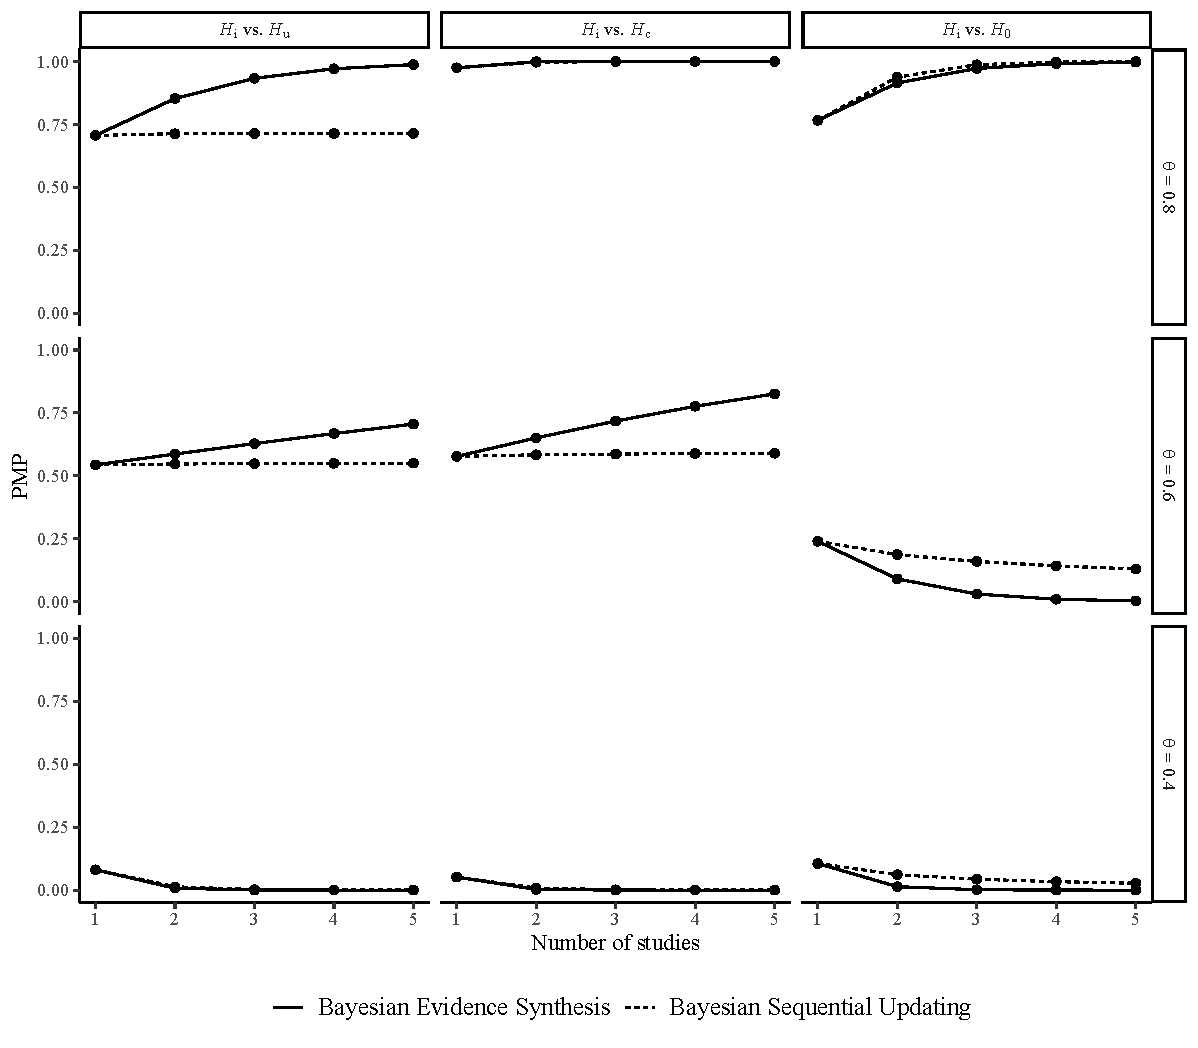
\includegraphics[width=14cm]{r-files-bes-klugkist-volker-2022/Figures/bes_bsu_pmp}}
 \caption{PMPs for BES (solid lines) and BSU (dashed lines) after combining 1-5 studies of $n=20$ with different effect sizes per row and testing $H_i: \theta>0.6$ against one of the alternatives $H_u: \theta$ (left), $H_c: \theta \leq 0.6$ (centre), $H_0: \theta=0.6$ (right). On the first row: $x/n=0.8$ and thus in agreement with $H_i$. On the second row: $x/n=0.6$ and thus in agreement with $H_0$. On the bottom row: $x/n=0.4$ and thus in agreement with $H_c$.}
 \label{aggre2}
\end{figure}

In Figure \ref{aggre2}, in the first row, results are plotted for the aggregation of evidence from 1 to 5 studies with success probability 0.8, that is, the data per study are in agreement with $H_i: \theta>0.6$. The increasing solid lines in the left, centre and right plot show the increasing amount of aggregated support when using BES with each of the three alternative hypotheses ($H_u$, $H_c$, $H_0$). We see that the current combination of effect size and sample size provides enough power for testing against $H_0$ in each study, and therefore also the aggregated support for $H_i$ increases with each new study. The almost horizontal line for testing against $H_c$, in the central plot on the first row, demonstrates that the support for $H_i$ against $H_c$ in this scenario approaches maximal support already with less than 5 studies.
Comparing the results with BSU, the dashed lines in the same plots, we see only a difference when evaluating against $H_u$. This is, again, explained by having a maximum value for the Bayes factor (and PMP) when testing against an unconstrained model.

In the second row, the observed effect in each sample is 0.6, which conforms exactly to the null hypothesis $H_0: \theta=0.6$. BSU results when testing against $H_u$ (left) or against $H_c$ (centre) show a stable indecisive result irrespective of adding more studies (horizontal dashed lines at PMP $\approx .5$). In contrast, BES shows a small increase in aggregated support for $H_i$ when adding more studies. Since $H_i$ is not 'the correct' hypothesis one could consider this an undesired result. The explanation is found in the fact that a Bayes factor balances fit and complexity and the two hypotheses compared (for both alternatives) differ in specificity. This is easiest explained looking at testing $H_i$ against $H_c$ (centre plot). The sample results with observed success rate of 0.6 provide approximately equal support, in terms of fit of data to the hypothesis, for $\theta>.6$ and $\theta<.6$. But $H_i: \theta>.6$ is more specific (containing 40$\%$ of the prior space) than $H_c$ (containing 60$\%$). This specificity effect accumulates over studies using BES, but not using BSU. In the plot on the right, both BSU and BES show a declining support for $H_i$ when tested against the in the data supported $H_0$. The gain in support in favor of the null hypothesis after synthesizing up to 5 studies is larger for BES than for BSU.

The last row presents the synthesized results when each study has success probability 0.4, that is, a result not in agreement with $H_i$, but instead in agreement with $H_c$. Irrespective of the alternative hypothesis, there is little support for $H_i$, as one would expect since each of the alternatives is more in line with the data than $H_i$ is. Both BSU and BES also show a further decrease in PMP values when adding more studies.






\subsection{An example of conceptual replications}\label{GLMexample}

In the previous section, we gave examples in which both BSU and BES could be applied. However, as previously discussed, when studies are methodologically diverse, using, for example, different operationalizations of key variables or different statistical models, BSU becomes inapplicable due to the fact that the estimated parameters are incomparable. It is, for instance, not at all straightforward to compare the effect of a key variable on a continuous outcome with the effect of this same variable on a dichotomous outcome. Yet, if both operationalizations represent the same construct, it is possible to quantify the support for the corresponding hypotheses in both studies, and aggregate the overall amount of evidence with BES. In the upcoming section, we present two simulation examples with such different operationalizations, both conducted in \texttt{R} \autocite[][Version 4.2.1]{R}.

\subsubsection{Simulation 1: Using BES when studies have different outcome variables}


In the first simulation, data is generated to represent three different studies using three different statistical models: ordinary least squares (OLS), logistic and probit regression.
In each study, a continuous or binary outcome $Y$ is regressed on five predictor variables $X_k$ ($k = 1,2,3,4,5$), that are normally distributed with mean $\mu_k = 0$, variance $\sigma^2_{k} = 1$ and common covariance $\rho_{k,k'} = 0.3$.
We consider the sample sizes $n = (50, 100, 200, 400, 800)$, and effect sizes $R^2 = (0.02, 0.09, 0.25)$, in accordance with small, medium and large effects, respectively, as defined by \textcite{cohen_1988}.
When the outcome of the study is continuous, the conventional $R^2$ is used, while for binary outcomes, McKelvey and Zavoina's $R^2_{M\&K}$ \autocite*{mckelvey_zavoina_1975} is used.
In each study, the relation between the predictors and the outcome variable is defined such that $\beta_1 = \beta_2 = \beta_3$, $\beta_4 = 2 \beta_1$ and $\beta_5 = 3\beta_1$.
The exact sizes of the coefficients depend on the effect size and the regression model used to generate the data (Appendix \ref{appendix:gendat} details how to calculate the coefficients for each model and effect size).
Based on the predictor variables and regression coefficients, the continuous outcomes are drawn from a normal distribution.
For dichotomous outcomes, the predictor variables and regression coefficients are first used to obtain success probabilities for each individual, after which the outcomes are drawn from a Bernoulli distribution (the exact procedure is described in Appendix \ref{appendix:gendat}).

For all combinations of effect and sample size, data is generated using OLS, logistic and probit regression models, to reflect three different studies.
In each of these studies, the focus is on the last three predictors, and the hypothesis $H_1: \beta_3 < \beta_4 < \beta_5$ is evaluated against its complement \autocite[using the \texttt{BF()} function from the \texttt{R}-package \texttt{BFpack}, with default (prior) settings;][Version 1.0.0]{BFpack}.
Subsequently, BES is used to aggregate the evidence for $H_1$ over these three studies.
The initial prior model probabilities are specified equally (i.e., $P(H_1) = P(H_{c}) = 0.5$).
This procedure is repeated over 1000 iterations for each combination of effect and sample size, to prevent that random fluctuations in data generation affect the conclusions.
The results are reported visually, in terms of the aggregated posterior model probabilities after incorporating the evidence from each of the three studies.
In these simulations, a combined PMP that is greater than $0.5$ reflects more support for the true hypothesis $H_1$ than for its complement $H_c$.

\begin{figure}[ht]
   \centerline{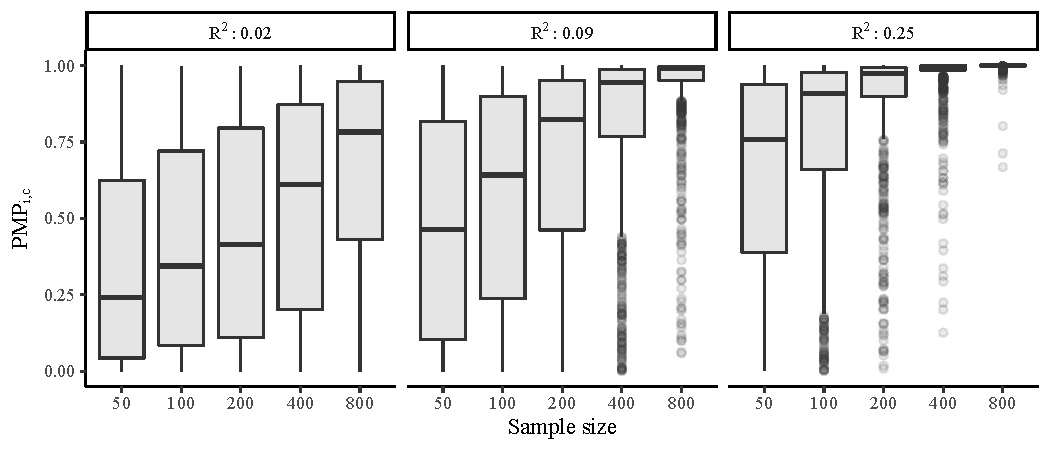
\includegraphics[width=15cm]{r-files-bes-klugkist-volker-2022/Figures/sim1_box}}
 \caption{Aggregated PMPs for the evidence for hypothesis $H_1: \beta_3 < \beta_4 < \beta_5$ against $H_c$ over three studies (based on OLS, logistic and probit regression models) for different combinations of effect and sample size.}
 \label{sim1_box}
\end{figure}

Figure \ref{sim1_box} shows that the support for the true hypothesis $H_1$ provided by BES increases with effect and sample size.
When the effect size is small, the support for $H_1$ varies considerably over the iterations, but hardly ever reaches convincing levels.
The same is true for the smallest sample size and a medium effect.
In these scenarios, each of the individual studies lack statistical power, regardless of the model used to generate the data.
For example, in Table \ref{pmp-studies} it is shown that the combination of the smallest effect size and smallest sample size yields a median PMP of about $.43$ in the individual studies (over 1000 iterations), with equivalent results for all three regression models.
Consequently, each of the studies contributes some support \textit{against} the hypothesis of interest, which accumulates when aggregating over studies.
Hence, when evaluating hypotheses on multiple parameters, BES requires sufficient statistical power, also when the alternative hypothesis of interest is not a classical null hypothesis (as presented in Section \ref{Binmultiple}) but a more general alternative hypothesis.
When the effect and sample sizes of the individual studies are sufficiently large, the aggregated support for $H_1$ is concentrated close to $1$, while there are less and less iterations that find little to no support.
Overall, these results again highlight that a lack of power in the individual studies accumulates when using BES.
When studies have sufficient power, BES can be applied to aggregate the evidence for theoretically equivalent hypotheses over heterogeneous studies.


\subsubsection{Simulation 2: Using BES when the studies have different predictors and outcome variables}

Simulation 2 builds on simulation 1, using the same sample sizes and effect sizes.
The outcome $Y$ is again continuous or binary, and is generated on the basis of the five predictor variables $X_1$ to $X_5$ using OLS, logistic and probit regression models.
The predictors of interest differ from simulation 1, as the focus is now on $X_1$, $X_2$ and $X_3$.
Moreover, simulation 2 exemplifies how BES can be used when not only the measurement level of the outcome variables, but also the operationalizations of the predictor variables differ.
Regardless of the operationalizations, which are manipulated after generating the data, it is assumed that $X_1$, $X_2$ and $X_3$ are different indicators of the same construct that is positively related to the outcome $Y$ ($H_2$).

In study $a$ the OLS model is used. Here, we consider the three distinct predictors separately, and thus hypothesize that $H_{2a}: \{\beta_1, \beta_2, \beta_3\} > 0$.
Study $b$ applies the logistic regression model. The three indicators are transformed into a scale score, by taking the mean of the three indicators for each observation, which is a common approach in the social sciences \autocite[e.g.,][]{bauer_discrepancy_2016}.
The corresponding hypothesis is that this scale score is positively related to the outcome $Y$, which yields $H_{2b}: \beta_{\text{scale}} > 0$.
In study $c$, generated and analyzed with probit regression, this operationalization is further adjusted.
The scale score that is used in study $b$ is categorized into three equally sized groups in each sample, corresponding to a \textit{low}, \textit{medium} and \textit{high} scoring group.
This is, despite common advice against it, common practice in many areas of research \autocite[e.g.,][]{bennette_against_2012, decoster_best_2011}.
The same expected positive relation between predictor and outcome now yields a specific ordering in the group means, resulting in hypothesis $H_{2c}: \beta_{\text{low}} < \beta_{\text{medium}} < \beta_{\text{high}}$.


\begin{figure}[ht]
   \centerline{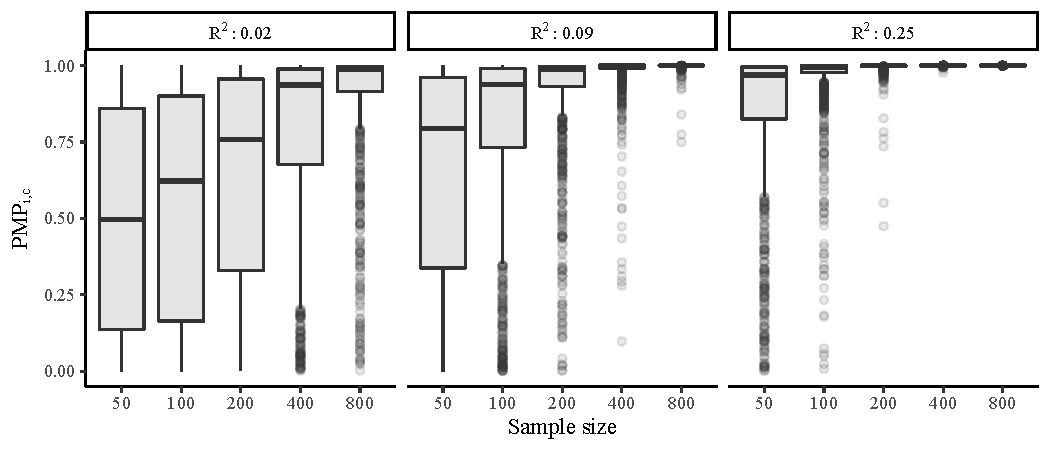
\includegraphics[width=14cm]{r-files-bes-klugkist-volker-2022/Figures/sim2_box}}
 \caption{Aggregated PMPs for the evidence for hypotheses $H_{2a}: \{\beta_1, \beta_2, \beta_3\} > 0$, $H_{2b}: \beta_{\text{scale}} > 0$ and $H_{2c}: \beta_{\text{low}} < \beta_{\text{medium}} < \beta_{\text{high}}$ against their respective complements over three studies (based on OLS, logistic and probit regression models) for different combinations of effect and sample size.}
\label{sim2_box}
\end{figure}


In simulation 2, the aggregated support for $H_2$ exceeds the support for its complement in the majority of the simulations for all effect and sample sizes, except for the combination of the smallest effect size with the smallest sample size.
In the latter case, the evidence is indecisive, with about equal support for both the hypothesis of interest and its complement.
The aggregated evidence for $H_2$ increases with effect size and sample size, and reaches substantial levels from relatively small sample and effect sizes onward.
For the largest effect size, the vast majority of the simulations results in relatively strong evidence for the overall hypothesis for all sample sizes.
Hence, although the study-specific hypotheses differ from study to study, the aggregated evidence supports the overall theory.


However, the aggregated results do not reveal how the individual studies contribute to this aggregate.
Whereas in the previous simulations, the considered hypothesis was identical over the different studies, the operationalization of the construct of interest, and thus the hypothesis under evaluation now varies over the three studies.
The hypotheses differ in the type and number of constraints, and therefore have different complexities.
At the same time, the different operationalizations affect the power of the performed analyses within each study.
Comparing the contributions of the individual studies indeed reveals that some operationalizations provide higher levels of support for the overall hypothesis than others (Table \ref{pmp-studies}).
Consistently over all combinations of effect and sample size, the data generated and analyzed with the logistic model, in which the separate indicators were averaged as a scale score, yielded the highest posterior model probabilities, and therefore contributed more to the aggregated evidence than the studies with OLS and probit data.
For example, for the smallest effect size and the smallest sample size in simulation 2, both the OLS and the probit study provide more support for the respective complement hypotheses, whereas only the logistic study provides evidence for the hypothesis of interest.
These results show that different ways of operationalizing the same theoretical construct affect the outcomes, but the final measure of BES does not reflect this variability. Hence, the individual studies provide valuable additional information.


\begin{table}[t]
\caption{Median posterior model probabilities for the individual studies and aggregated over studies in simulation 1 and 2, for a selection of effect sizes and sample sizes.}
\label{pmp-studies}
\centering
\begin{tabular}{lrrrrrrr}
\hline
Simulation & $R^2$ & Sample size & OLS & Logistic & Probit & & Aggregated \\
\hline
1 & $0.02$ & 50 & 0.44 & 0.43 & 0.42 & & 0.24 \\
  & $0.02$ & 200 & 0.52 & 0.50 & 0.50 & & 0.42 \\
  & $0.02$ & 800 & 0.65 & 0.61 & 0.62 & & 0.78 \\
\hline
1 & $0.25$ & 50 & 0.66 & 0.61 & 0.59 & & 0.76 \\
  & $0.25$ & 200 & 0.81 & 0.79 & 0.76 & & 0.97 \\
  & $0.25$ & 800 & 0.96 & 0.93 & 0.91 & & 1.00 \\
\hline
2 & $0.02$ & 50 & 0.45 & 0.62 & 0.49 & & 0.50 \\
  & $0.02$ & 200 & 0.58 & 0.69 & 0.54 & & 0.76 \\
  & $0.02$ & 800 & 0.75 & 0.90 & 0.71 & & 0.99 \\
\hline
2 & $0.25$ & 50 & 0.75 & 0.87 & 0.65 & & 0.97 \\
  & $0.25$ & 200 & 0.93 & 0.98 & 0.86 & & 1.00 \\
  & $0.25$ & 800 & 1.00 & 1.00 & 0.98 & & 1.00 \\
\hline
\end{tabular}
\end{table}


\section{Conclusion and discussion}
\label{Concl}

In this paper we explained BES, a relatively novel method for combining evidence from (conceptual) replications. One of the appealing characteristics of BES is that it does not require similar operationalizations in different studies. As long as the theory of interest can be formalized as an informative hypothesis, the support for the theory in each study can be expressed in terms of a Bayes factor, and BES can be applied to synthesize the evidence for this theory over studies. Especially in the context of conceptual replications, variability in research designs, for instance in terms of operationalizations and analysis models, is encouraged to enhance the validity of the drawn conclusions or to provide insight in the required conditions for the conclusions to hold. As such variability renders a synthesis at the level of model parameters or effect sizes infeasible, BES provides a flexible alternative to conventional approaches for a quantitative synthesis of the evidence for the overall theory.

To illustrate the behavior of BES we first demonstrated the aggregation of multiple studies with the exact same result in each sample. This scenario represents the situation of exact replications and therefore allowed for a comparison of results from BES with BSU. Using a simple binomial model that could be analyzed analytically, we computed Bayes factors for an informative hypothesis against one of three typical alternatives: the unconstrained, the complement and the null hypothesis. 

The results demonstrated that both methods behave well in the sense that larger sample sizes, larger effect sizes, and more aggregated studies generally increase the support for the best hypothesis. However, we also demonstrated that the two methods of aggregation provide answers to different questions. BSU pools all available data and thus provides the support for the hypothesis of interest in all studies when taken together. This increases the total sample size and thus statistical power to find support for the true hypothesis, which is usually considered a strength of this method. BES, on the other hand, measures the level of aggregated evidence in a different way, by first determining the evidence in each study and then combining the support levels over studies. This implies, for instance, that if two underpowered studies each provide most support for the null hypothesis, the aggregated evidence using BES results in even stronger support for the null. This can be considered a disadvantage of BES: it is not a remedy against underpoweredness. 

The main strength of BES is its flexibility. Results of highly diverse studies can be aggregated in a simple straightforward way by updating posterior odds with each additional study. This was demonstrated in the two simulation studies in this paper. In the first simulation, the three studies that were aggregated differed in the outcome variable and corresponding statistical model, while the formulation of the informative hypothesis was equal for all studies. Repeated sampling of data representing these three studies and, in each repetition, aggregating evidence over the three studies demonstrated that BES can indeed aggregate evidence from diverse studies and showed, again, that the performance of BES is generally as one would expect. Larger samples and larger effect sizes lead to higher levels of support for the hypothesis that reflects the true population effect. It also showed that a lack of power in the individual studies accumulates when using BES. Where in the 'one parameter with one constraint' binomial example, we only encountered power issues for testing against the null hypothesis, this simulation with a hypothesis with multiple constrained parameters showed similar issues when testing against a more general alternative hypothesis. 

The second simulation used a similar set-up for sampling data for the different statistical models but now also changed the formulation of predictors, in such a way that different informative hypotheses represented the general hypothesis. The results showed that with these different operationalizations, some studies provided higher levels of support for the theory than others. For example, collapsing the three indicators into a single scale score increased the statistical power of the analysis, and thus contributed more strongly to the aggregated evidence than the study that included the separate indicators. Another difference between the hypotheses of the individual studies was the number of constraints imposed on the regression parameters, in order to represent the general theory of interest. Since the type and number of constraints determine the complexity of a hypothesis, and since the Bayes factor depends not only on the fit of the data to the hypothesis but also on this complexity, these differences have an impact on the level of support reached within a study. Table 3 in this paper gives a first impression of the impact of differences in informative hypotheses on resulting Bayes factors, but more research into this effect and to what extent this may be problematic for the aggregation is needed. 


In conclusion, we believe that BES provides a valuable and unique tool for the aggregation of evidence from a heterogenous set of studies. It generally performs well, although certain issues require further attention. 
The simulation studies in this paper were merely for illustrative purposes to get an impression on what BES has to offer, however, they also provided cues on what still needs to be investigated further in a more comprehensive evaluation of the performance of BES. For instance, users need to be aware that if one or more of the aggregated studies lack power, BES does not provide a solution for this underpoweredness because it is not a data-pooling approach. The Bayes factor in the underpowered study will provide most support for the most parsimonious hypothesis, and BES will take that support measure into account when aggregating evidence from multiple studies. A second issue that needs attention is that Bayes factors are not only affected by the fit of the data to the hypothesis (including the impact of effect sizes and sample sizes) but also to the complexity of the hypothesis. Hypotheses that are more specific (i.e., with a smaller complexity) will, with the same fit, provide larger Bayes factor values and thus have a stronger impact on the aggregated evidence. To what extent or under which circumstances this is desirable or problematic requires more research into different scenarios. Also, the impact of aggregating studies with considerable differences in sample size is a relevant topic for future research. In the examples and simulations of this paper, we always aggregated evidence levels from studies of the same size. In practical applications, this is usually not the case and it is important to understand how this impacts the behavior of BES.

Our final remark is about the position of this paper in the existing literature. Although we consider this work to be an introduction of the BES approach and have written it for potential users who are new to the method, it is not the first paper about BES. It all started with the work by \textcite{kuiper_combining_2013}. They introduced the method for the evaluation of a hypothesis constraining one regression parameter to be positive within different statistical models, applied in the context of sociological research. Since then, BES has been applied in a few psychological studies \autocite{zondervan_parental_2019, zondervan_robust_2020, kevenaar_bes_2021} and a sociological study \autocite{volker_cooperation_2022}, and is described in a paper providing an overview of different methods using Bayes factors \autocite{heck_review_2022}. Only recently, we started studying BES under more varied circumstances to better understand its behavior. This led to two more papers written more or less in parallel with this introductory paper \autocite[][submitted for publication and available online]{vanwonderen_bes_2022, volker_bes_2022}. We feel that to be able to properly evaluate and value BES, the current paper provides a good starting point.





\printbibliography

\begin{appendices}
\section{Data generation and analysis} \label{appendix:gendat}

In this appendix, the data-generating mechanisms of the two simulations are outlined in more (mathematical) detail.

\subsection{Simulation 1}

In simulation 1, data is generated to represent three different studies with different outcome variables, but with the same set of predictor variables.
For each of these three studies, a different statistical model is used to generate the data: ordinary least squares (OLS), logistic and probit regression.
Under OLS, the outcome variable $Y$ is continuous, whereas for logistic and probit regression, $Y$ is binary.
In each study, $Y$ is related to the $n \times 5$ predictor matrix $X$, where each predictor $X_k$
is normally distributed with mean $\mu_k = 0$, variance $\sigma_k^2 = 1$ and common covariance $\rho_{k, k'} = 0.3$.
Accordingly, the mean vector $\mu$ and covariance matrix $\Sigma$ are defined as
\begin{equation}
\mu = \begin{bmatrix} 0 \\ 0 \\ 0 \\ 0 \\ 0 \\ \end{bmatrix}, ~~~~~~
\Sigma = \begin{bmatrix}
1 & 0.3 & 0.3 & 0.3 & 0.3 \\
0.3 & 1 & 0.3 & 0.3 & 0.3 \\
0.3 & 0.3 & 1 & 0.3 & 0.3 \\
0.3 & 0.3 & 0.3 & 1 & 0.3 \\
0.3 & 0.3 & 0.3 & 0.3 & 1 \\
\end{bmatrix}.
\end{equation}
Throughout the simulations, we consider the sample sizes $n = (50, 100, 200, 400, 800)$ and effect sizes $R^2 = (0.02, 0.09, 0.25)$, corresponding to Cohen's \autocite*{cohen_1988} definition of small, medium and large effects, respectively.
Note that the regular $R^2$ is used for data generated by OLS regression, whereas McKelvey and Zavoina's $R^2_{M\&K}$ \autocite*{mckelvey_zavoina_1975} is used for data generated with logistic and probit regression. This measure closely resembles the conventional $R^2$ empirically \autocite{hagle_mitchell_goodness_1992, demaris_explained_2002}.
Based on these effect sizes, one can define the variance of the linear predictor $\text{Var}(\hat{Y})$, where $\hat{Y} = X\beta$ and $\beta$ denotes the column vector with regression coefficients.
When $Y$ is continuous with variance $\sigma^2_Y = 1$ (which is the case in our simulations), the variance of the linear predictor is equal to the effect size (i.e., $\text{Var}(\hat{Y}) = R^2$).
For logistic regression, $\text{Var}(\hat{Y}) = \frac{R^2 \frac{\pi^2}{3}}{1-R^2}$, and for probit regression $\text{Var}(\hat{Y}) = \frac{R^2}{1 - R^2}$.

The relationship between each predictor $X_k$ and the outcome $Y$ is specified such that $\beta_1 = \beta_2 = \beta_3$, $\beta_4 = 2\beta_1$ and $\beta_5 = 3\beta_1$.
These relationships are captured in the column vector $B = \begin{bmatrix} 1 & 1 & 1 & 2 & 3 \end{bmatrix}'$.
Based on the relative size of the regression coefficients as specified in $B$, the variance of the linear predictor $\text{Var}(\hat{Y})$ defined as function of effect size $R^2$ and the covariance-matrix of the predictors $\Sigma$, the exact size of the regression coefficients $\beta$ is defined as
\begin{equation}
\beta = B \Bigg(\sqrt{\frac{\text{Var}(\hat{Y})}{G' ((B B') \odot \Sigma) G }}\Bigg),
\end{equation}
where $G = \begin{bmatrix} 1 & 1 & 1 & 1 & 1 \end{bmatrix}'$ and $\odot$ denotes the Hadamard element-wise product. The resulting coefficients are reported in Table \ref{coefs}.
Continuous outcomes are drawn from a normal distribution
\begin{equation}
Y \sim \mathcal{N}(X\beta, 1 - R^2),
\end{equation}
with mean vector $X \beta$ and residual variance $\sigma_{\epsilon}^2 = 1 - R^2$.
Binary outcomes are drawn from a Bernoulli distribution
\begin{equation}
Y \sim \mathcal{B}(p),
\end{equation}
where $p$ equals
\begin{equation}
p_{\text{logistic}} = \frac{1}{1 + e^{-X\beta}},
~~~~~~~~~
p_{\text{probit}} = \Phi(X\beta),
\end{equation}
for logistic and probit regression, respectively, and with $\Phi$ indicating the cumulative normal distribution.

\begin{table}[t]
\centering
\caption{Population-level regression coefficients for ordinary least squares (OLS), logistic and probit regression, given effect sizes of $R^2 \in \{0.02, 0.09, 0.25\}$.}
\label{coefs}
\begin{tabular}{lllllllllllll}
  \toprule
  $R^2$ & & \multicolumn{3}{c}{OLS} & & \multicolumn{3}{c}{Logistic} & & \multicolumn{3}{c}{Probit} \\
 \midrule
  &   & $\beta_{1, 2, 3}$ & $\beta_4$ & $\beta_5$ &   & $\beta_{1, 2, 3}$ & $\beta_4$ & $\beta_5$ &   & $\beta_{1, 2, 3}$ & $\beta_4$ & $\beta_5$ \\
   \midrule
0.02 &   & 0.026 & 0.051 & 0.077 &   & 0.047 & 0.094 & 0.141 &   & 0.026 & 0.052 & 0.078 \\
  0.09 &   & 0.054 & 0.109 & 0.163 &   & 0.103 & 0.207 & 0.310 &   & 0.057 & 0.114 & 0.171 \\
  0.25 &   & 0.091 & 0.181 & 0.272 &   & 0.190 & 0.380 & 0.570 &   & 0.105 & 0.209 & 0.314 \\
   \bottomrule
\end{tabular}
\end{table}

Subsequently, each study is analyzed with an OLS, logistic or probit regression model, in which the outcome $Y$ is regressed on all $5$ predictors and an intercept (which equals 0 in the population).
In each study, the same hypothesis $H_1: \beta_3 < \beta_4 < \beta_5$ is evaluated against its complement using the \texttt{BF()} function from the \texttt{R}-package \texttt{BFpack} \autocite[][Version 1.0.0]{BFpack}, using default (prior) settings.
After analyzing the three individual studies, the results are aggregated using BES. 
The initial prior model probabilities are specified equally (i.e., $P(H_1) = P(H_0) = 0.5$).
This entire procedure (data generation and analysis of each of the three individual studies, and aggregating with BES) is repeated over 1000 iterations for each combination of effect and sample size.

\subsection{Simulation 2}

The data in simulation 2 is generated in exactly the same way as in simulation 1, using the same statistical models, combinations of effect and sample size, and the same predictor specifications.
What is different, is that in simulation 2, interest is in the effects of the first three predictor variables, which are regarded as indicators of the same theoretical construct.
A positive relation between this construct and the outcome $Y$ is expected in all three studies, but the operationalizations of this construct differs between studies.
This data manipulation is performed after generating the data.

Study $a$ employs OLS regression, and considers the three indicators separately, such that the hypothesis of interest states that $H_{2a}: \{\beta_1, \beta_2, \beta_3\} > 0$.
The regression model that is fitted to the data contains all five predictor variables and an intercept.
Study $b$ employs logistic regression, and the construct of interest is operationalized as a scale score, that is created by taking the mean of the three indicators for each observation, such that $X_{\text{scale}} = (X_1 + X_2 + X_3)/3$.
The hypothesis of interest is thus formalized as $H_{2b}: \beta_{\text{scale}} > 0$.
In this study, the effects of $X_{\text{scale}}$ and the variables $X_4$ and $X_5$ on $Y$ are modeled, and an intercept is included.
In study $c$, which uses probit regression, the scale score from study $b$ is categorized into three groups.
Each group contains $1/3$ of the observations in each sample, corresponding to \textit{low}, \textit{medium} and \textit{high} scoring groups.
Here, the expected positive relation between the construct of interest and $Y$ yields a specific ordering of the group means, resulting in hypothesis $H_{2c}: \beta_{\text{low}} < \beta_{\text{medium}} < \beta_{\text{high}}$.
The regression model that is used to analyze this data contains these three dummy variables and the variables $X_4$ and $X_5$, and thus no intercept (this information is contained within these dummies).
Each of the hypotheses ($H_{2a}$, $H_{2b}$ and $H_{2c}$) is evaluated against its respective complement.
Similarly to simulation 1, BES is applied to aggregate the support for the overall hypothesis $H_2$ over these studies, again using equal initial prior model probabilities.
This process is repeated over 1000 iterations for each combination of effect and sample size.


\end{appendices}
\end{document}






